\section{Auswertung}
\label{sec:Auswertung}
Die Tabelle \ref{tab:1} enthält die Messwerte für die Kennlinienschar
bei unterschiedlichen Heizströmen $I_{f}$ und Heizspannungen $U_f$.
\begin{align*}
\intertext{Messung 1:}  I_f&=2,5\si{\ampere} \ \ \ \ &V_f=6,5\si{\volt}\\
\intertext{Messung 2:}  I_f&=2,4\si{\ampere} \ \ \ \ &V_f=6,0\si{\volt}\\
\intertext{Messung 3:}  I_f&=2,3\si{\ampere} \ \ \ \ &V_f=5,5\si{\volt}\\
\intertext{Messung 4:}  I_f&=2,2\si{\ampere} \ \ \ \ &V_f=5,2\si{\volt}\\
\intertext{Messung 5:}  I_f&=2,1\si{\ampere} \ \ \ \ &V_f=5,0\si{\volt}
\end{align*}


\begin{table}
  \centering
  \caption{.}
  \label{tab:1}
  \begin{tabular}{c c c c c c}
  \toprule
  Anodenspannung &  Messung 1 & Messung 2 & Messung 3 & Messung 4 & Messung 5\\ %\multicolumn{2}{c}{Verhältniss}\\
  $V/\si{\volt}$ & $I_1/\si{\milli\ampere}$ & $I_2/\si{\milli\ampere}$ &$ I_3/\si{\milli\ampere}$ &$I_4/\si{\milli\ampere}$ & $I_5/\si{\milli\ampere}$\\
  \midrule
  0   & 0,000 &  0,000 &  0,000 &  0,000 &  0,000    \\
  5   & 0,013 &  0,017 &  0,016 &  0,013 &  0,011\\
  10  & 0,033 &  0,035 &  0,033 &  0,031 &  0,027\\
  15  & 0,053 &  0,053 &  0,053 &  0,052 &  0,043\\
  20  & 0,079 &  0,080 &  0,075 &  0,071 &  0,061\\
  25  & 0,108 &  0,109 &  0,101 &  0,094 &  0,079\\
  30  & 0,143 &  0,140 &  0,130 &  0,120 &  0,097\\
  35  & 0,179 &  0,175 &  0,164 &  0,148 &  0,117\\
  40  & 0,216 &  0,210 &  0,195 &  0,176 &  0,135\\
  45  & 0,261 &  0,247 &  0,226 &  0,206 &  0,155\\
  50  & 0,300 &  0,289 &  0,264 &  0,234 &  0,170\\
  55  & 0,360 &  0,337 &  0,302 &  0,266 &  0,187\\
  60  & 0,433 &  0,383 &  0,348 &  0,299 &  0,200\\
  70  & 0,524 &  0,490 &  0,436 &  0,461 &  0,214\\
  80  & 0,638 &  0,598 &  0,519 &  0,425 &  0,232\\
  90  & 0,759 &  0,674 &  0,602 &  0,576 &  0,243\\
  100 & 0,866 &  0,818 &  0,665 &  0,524 &  0,272\\
  110 & 1,029 &  0,923 &  0,743 &  0,562 &  0,290\\
  120 & 1,155 &  1,055 &  0,813 &  0,595 &  0,299\\
  130 & 1,298 &  1,165 &  0,883 &  0,622 &  0,306\\
  140 & 1,450 &  1,282 &  0,954 &  0,645 &  0,312\\
  150 & 1,601 &  1,394 &  1,011 &  0,664 &  0,319\\
  160 & 1,769 &  1,511 &  1,056 &  0,678 &  0,325\\
  170 & 1,920 &  1,623 &  1,097 &  0,687 &  0,330\\
  180 & 2,080 &  1,739 &  1,134 &  0,694 &  0,334\\
  190 & 2,220 &  1,852 &  1,175 &  0,700 &  0,337\\
  200 & 2,390 &  1,956 &  1,207 &  0,705 &  0,340\\
  210 & 2,550 &  2,060 &  1,232 &  0,709 &  0,342\\
  220 & 2,710 &  2,140 &  1,251 &  0,714 &  0,345\\
  230 & 2,880 &  2,250 &  1,267 &  0,718 &  0,347\\
  240 & 3,050 &  2,340 &  1,282 &  0,718 &  0,349\\
  250 & 3,110 &  2,440 &  1,294 &  0,721 &  0,350\\
  \bottomrule
 \end{tabular}
\end{table}
\FloatBarrier

Diese Messwerte werden nun in der Abbildung \ref{fig:1} in der Form
Annodenstrom $I$ in Abhängigkeit von der Annodenspannung $U$
aufgetragen.

\begin{figure}
 \centering
 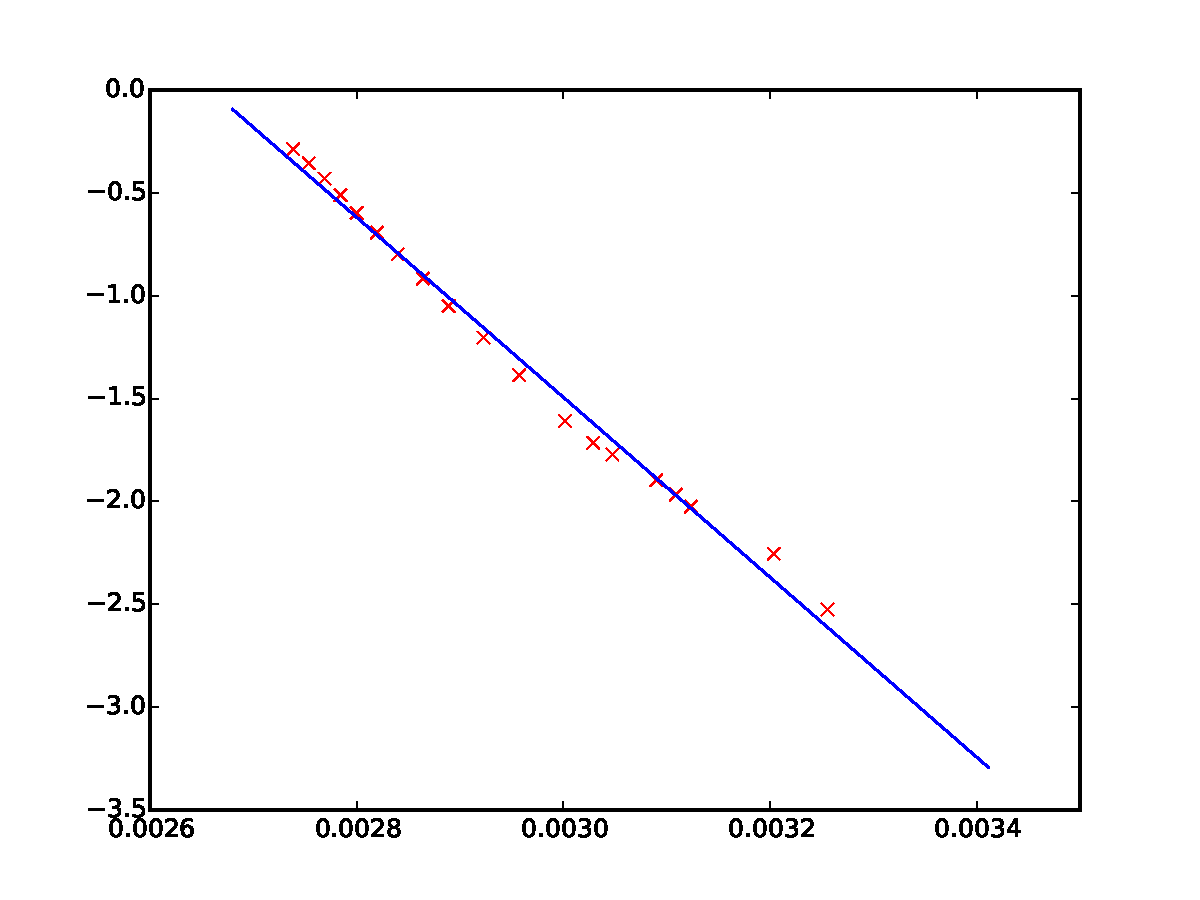
\includegraphics[width=0.7\textwidth]{plot1.pdf}
 \caption{Der gemessene Annodenstrom $I$ in Abhängigkeit von der Annodenspannung $U$}
 \label{fig:1}
\end{figure}
\FloatBarrier

Aus der der Abbildung \ref{fig:1} und der Tabelle \ref{tab:1}
kann für jede Heizspannung $I_f$ der
Sättigungsstrom $I_S$ abgelesen werden.
Die Tabelle \ref{tab:I_s} enthält die entsprechenden Werte für den Sättigungsstrom $I_S$.
\begin{table}
  \centering
  \caption{Die Sättigungsströme $I_S$ der einzelnen Messungen.}
  \label{tab:1}
  \begin{tabular}{c c c c c c}
  \toprule
   &  Messung 1 & Messung 2 & Messung 3 & Messung 4 & Messung 5\\ %\multicolumn{2}{c}{Verhältniss}\\
   \midrule
  $I_S/\si{\milli\ampere}$ & 3,110 & 2,440  & 1,294 & 0,721 & 0,350?? \\
  \bottomrule
  \end{tabular}
\end{table}
\FloatBarrier

Nun wird für die maximale Heizleistung $I_f=2,5\si{\ampere}$
das Raumladungsgebiet abgeschätzt.
Dieses lässt sich aus der Abblidung \ref{fig:fitt} abschätzen
und liegt ungefähr zwischen $0\si{volt}$ und $170\si{\volt}$.
\begin{figure}
 \centering
 \includegraphics[width=0.7\textwidth]{plotfitt.pdf}
 \caption{Der gemessene Annodenstrom $I$ in Abhängigkeit von der Annodenspannung $U$ bei maximaler
Heizleistung. Sowie die Ausgleichsfunktion für das Raumladungsgebiet.}
 \label{fig:fitt}
\end{figure}
\FloatBarrier

Für das Raumladungsgebiet soll der Zusammenhang
zwischen der Annodenspannung $U$ und dem Annodenstrom $I$ untersucht
werden.
Dabei wird versucht ein Ausgleichsfunktion, der Form
\begin{align}
  I=a\cdot U^{b},
\end{align}
an die Messwerte aus dem Raumladungsgebiet zu fitten.
Es ergeben sich die folgenden Koeffizienten:
\begin{align*}
a=(9,64\pm0,38)\cdot10^{-10}\si{\ampere\per\volt}
b=(1,48\pm0,01)
\end{align*}




\subsection{Anlaufstromgebiet}
In der Tabelle \ref{tab:2} sind die gemessenen Anlaufström $I_A$
und die Gegenspannung $U_g$ aufgelistet.
Um nun mit Hilfe einer Ausgleichsfunktion die Kathodentemperatur $T$
zu berechnen, muss der Spannungsverlust
\begin{align*}
  \Delta U=R_i\cdot I_A
\end{align*}
and dem nA-Meter, welches einen Innenwiederstand $R_i=1\si{\mega\ohm}$ besitzt,
berücksichtigt werden.
Die Korriegierte Spannung $U_k$ ergibt sich somit aus
\begin{align}
U_k=U_g-R_i\cdot I_A \label{eqn:U_k}
\end{align}
und ist ebenfalls in der Tabelle \ref{tab:2} enthalten.

\begin{table}
  \centering
  \caption{.}
  \label{tab:2}
  \begin{tabular}{c c c}
  \toprule
  Gegenspannung  & Anodenstrom & korriegierte Gegenspannung\\ %\multicolumn{2}{c}{Verhältniss}\\
  $U_g/\si{\volt}$ & $I_A/\si{\nano\ampere}$ & $U_k/\si{\milli\volt}$\\
   \midrule
0     &  9,5  & -9,5\\
0,05  &  7,3  & 42,7\\
0,1   &  5,5  & 94,45\\
0,15  &  4,45 & 145,55\\
0,2   &  3,4  & 196,66\\
0,25  &  2,65 & 247,35\\
0,3   &  2,05 & 297,95 \\
0,35  &  1,50 & 348,5\\
0,4   &  1,2  & 398,8\\
0,45  &  0,9  & 449,1\\
0,5   &  0,89 & 499,11\\
0,55  &  0,69 & 549,31\\
0,6   &  0,55 & 599,45\\
0,65  &  0,42 & 649,58\\
0,7   &  0,34 & 699,66\\
0,75  &  0,27 & 749,73\\
0,8   &  0,22 & 799,78\\
0,85  &  0,18 & 849,82\\
0,9   &  0,15 & 899,85\\
0,95  &  0,13 & 949,87\\
\bottomrule
\end{tabular}
\end{table}
\FloatBarrier
%
Wird nun der Strom $I_A$ halblogarithmisch gegen
die korriegierte Gegenspannung $U_k$ aufgetragen
wie in Abbildung \ref{fig:log}

\begin{figure}
 \centering
 \includegraphics[width=0.7\textwidth]{plotanlauf.pdf}
 \caption{Der Anlaufstrom $I_A$  halblogarithmisch gegen
 die korriegierte Gegenspannung $U_k$ aufgetragen. }
 \label{fig:log}
\end{figure}

Über eine Lineareregression und der Formel \eqref{eqn:Pot}kann die Kathodentemperatur $T$
berechnet werden.
Es ergeben sich die Folgenden werte:
\begin{align*}
m=-4,51\pm0,06\\
b=-18,62\pm0,03
\intertext{Die Steigung $m$ entspricht dabei}
  m=-\frac{e_0}{k\cdot T}.
\intertext{Daraus folgt}
T=-\frac{e_0}{k\cdot m}.
\intertext{Somit beträgt die Kathodentemperatur}
T=(2573\pm35)\si{\kelvin}.
\end{align*}

\subsection{Leistungsbilanz}
Ebenfalls dann die Kathodentemperatur $T$ auch über die
Leistungsbilanz der Heizstromkreises berechnen.
Dafür werden die gegebenen Werte in Gleichung \eqref{eqn:leistung}
eingesetzt und nach $T$ umgestellt.
\begin{align}
I_f\cdot U_f=f\eta\sigma T^4- N_{WL} \label{eqn:leistung}
\end{align}
Dabei ist $f$ die Kathodenoberfäche
\begin{align*}
  f=0,32\si{\centi\meter\tothe{2}},
\intertext{$\eta$ der Emissiongrad der Oberfläche}
  \eta=0,28,
\intertext{$\sigma$ die Stefan-Boltzmannsche Strahlungskonstante}
 \sigma=5,7\cdot10^{-12}\si{\watt\per\centi\meter\tothe{2}\kelvin\tothe{4}},
\intertext{und $N_{WL}$ die abeschätzte Wärmeleitung der Apparatur}
N_{WL}=0,9\si{\watt}.
\end{align*}
Es ergibt sich eine Kathodentemperatur von
\begin{align*}
  T=2235\si{\kelvin}
\end{align*}
